\chapter{Antibody example with a double pendulum}
\label{app:AntiBody}
%
In this appendix the equation of motion of a double pendulum are derived with two approach: the standard one and the antibody one.\\
Lets suppose to have a double pendulum in figure \ref{fig:DoublePendulum} whose arm are of length $L_1$ and $L_2$. The motion of the two bodies can be describe using a minimum set of coordinate which are the two angles $\theta_1(t)$ and $\theta_2(t)$. Using the multibody approach one can define the body of the fist link attached to a reference frame ($\it RF_1$) rotated of $\theta_1(t)$, with the CoM in $G_1$ and having mass $m_1$ and inertia $Iz_1$. In the same way one can derive a reference frame $\it RF_2$ translating from $\it RF_1$ along the link 1 of $L_1$ and rotating of the relative angle $\theta_2(t)$. From that one can define a body, link 2, with mass $m_2$ and inertia $Iz_2$ in the CoM $G_2$.
%
\begin{figure}[ht!]
    \centering
    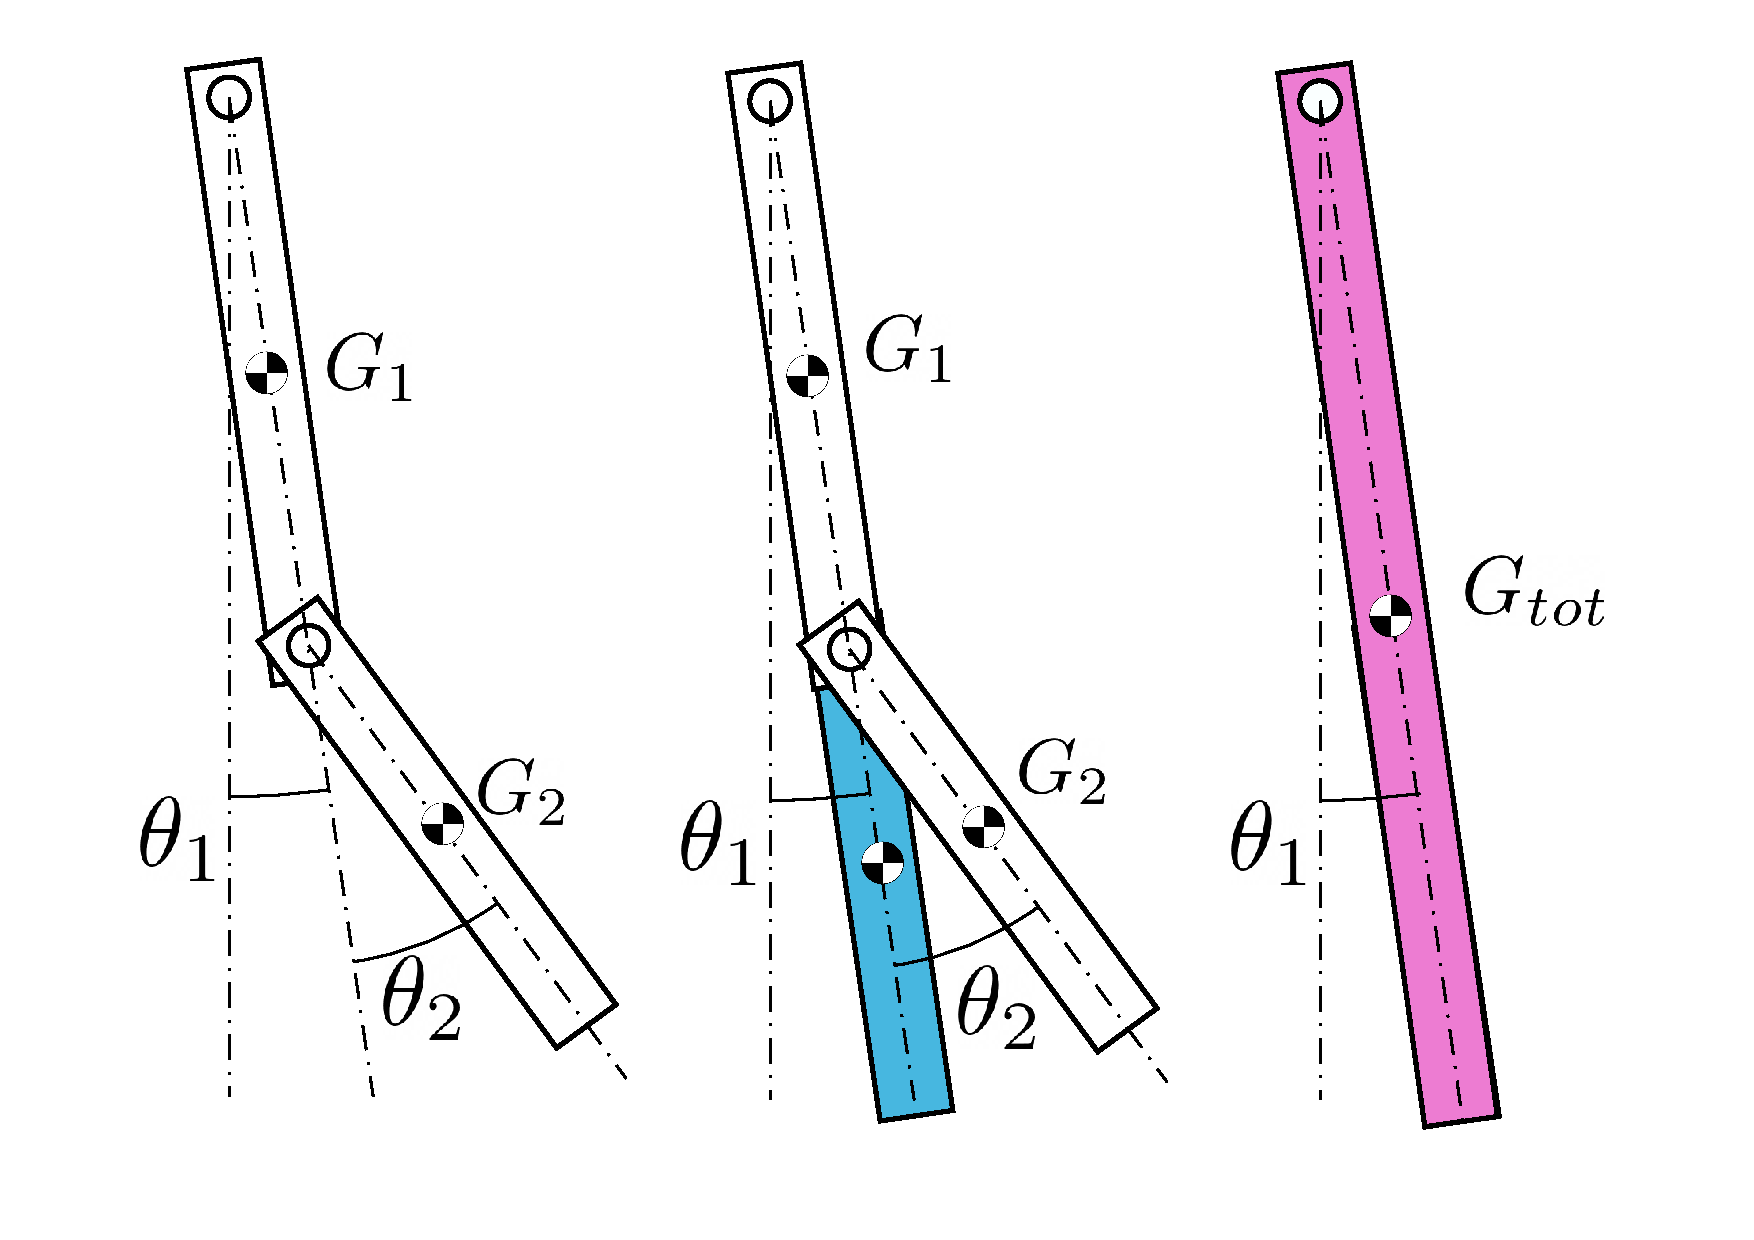
\includegraphics[width=\linewidth]{Coordinates/DPendulum.pdf}
    \caption{Double pendulum, in light blue the anti body and in purple the link sum of link 1 and 2}
    \label{fig:DoublePendulum}
\end{figure}
%
\section{Straight forward derivation}
%
Using the lagrange approach one can write down the kinetic and the potential energy of the system of two body and retrieve the following expression.
%
\footnotesize
\begin{equation}
    \label{eq:lagrange}
\begin{cases}
    \begin{split}
& \left( 2\,Lm_{2}\,{\it xg}_{2}\,\cos\left( \theta_{2} \left( t \right)  \right) + \left( {L}^{2}+{{\it xg }_{2}}^{2} \right) m_{2}+m_{1}\,{{\it xg}_{1}}^{2}+{\it iz}_{1}+{\it iz}_{2} \right) {\frac {{\rm d}^{2}}{{\rm d}{t}^{2}}}\theta_{1}\left( t \right) + \dots \\
&\quad\dots + \left( {\frac {{\rm d}^{2}}{{\rm d}{t}^{2}}}\theta_{2} \left( t \right)  \right)  \left( Lm_{2}\,{\it xg}_{2}\,\cos\left( \theta_{2} \left( t \right)  \right) +m_{2}\,{{\it xg}_{2}}^{2}+{\it iz}_{2} \right) + \dots\\
&\quad\dots - \left( {\frac {\rm d}{{\rm d}t}}\theta_{2}\left( t \right)  \right) ^{2}Lm_{2}\,{\it xg}_{2}\,\sin \left( \theta_{2} \left( t \right)  \right) -2\,Lm_{2}\,{\it xg}_{2}\,\left( {\frac {\rm d}{{\rm d}t}}\theta_{2} \left( t \right)  \right) \sin \left( \theta_{2} \left( t \right)  \right) {\frac {\rm d}{{\rm d}t}}\theta_{1} \left( t \right) + \dots \\
&\quad \dots + g \left( \cos \left( \theta_{2}\left( t \right)  \right) \sin \left( \theta_{1} \left( t \right) \right) m_{2}\,{\it xg}_{2} + \left( Lm_{2}+m_{1}\,{\it xg}_{1}\right) \sin \left( \theta_{1} \left( t \right)  \right) + \sin\left( \theta_{2} \left( t \right)  \right) \cos \left( \theta_{1}\left( t \right)  \right) m_{2}\,{\it xg}_{2} \right) 
\end{split}\\
\begin{split}
&\left( Lm_{2}\,{\it xg}_{2}\,\cos \left( \theta_{2} \left( t \right)  \right) +m_{2}\,{{\it xg}_{2}}^{2}+{\it iz}_{2}\right) {\frac {{\rm d}^{2}}{{\rm d}{t}^{2}}}\theta_{1} \left( t\right) + \left( {\frac {{\rm d}^{2}}{{\rm d}{t}^{2}}}\theta_{2}\left( t \right)  \right)  \left( m_{2}\,{{\it xg}_{2}}^{2}+{\it iz}_{2} \right) + \dots \\
&\quad \dots + {\it xg}_{2}\,m_{2}\, \left( L \left( {\frac {\rm d}{{\rm d}t}}\theta_{1} \left( t \right)  \right) ^{2}\sin \left( \theta_{2} \left( t \right)  \right) +g \left( \sin \left( \theta_{1} \left( t \right)  \right) \cos \left( \theta_{2} \left( t \right)  \right) +\cos \left( \theta_{1} \left( t \right)  \right) \sin \left( \theta_{2} \left( t \right)  \right)  \right)  \right)  
\end{split}  
\end{cases} 
\end{equation}
\normalsize
%
\section{Dummy body techniques}
%
In order to use the dummy body technique one should define the antibody as a body with negative massa and inertia. In this case the only antibody needed is the one of link 2, considering the internal DoF $\theta_2(t)$ as zero.\\
The next step is to define a body which is the sum of the two links with the internal DoF. This body will have a mass $M$ equal to the sum of the two masses ($m_1+m_2$).\\
The CoM will be in the coordinate $\it YG$ calculated as the weighted sum of the CoMs $G_1$, $G_2$.
%
\begin{equation}
    {\it YM} = \frac{-L_1 m_2-m_1 {\it yg_1}-m_2 {\it yg_2}}{m_1+m_2}
\end{equation}
%
The inertia $\it IZ$ can be retrieved considering the angular momentum of the two bodies (link 1 and link 2).
%
\begin{equation}
    {\it IZ} =  (L_1 m_2+m_1 {\it yg_1}+m_2 {\it yg_2}) {\it YG}+L_1^2 m_2+2 L_1 m_2 {\it yg_2}+m_1 {\it yg_1}^2+m_2{\it yg_2}^2+{\it iz_1}+{\it iz_2}
\end{equation}
%
Finally one can derive the equation of motion using lagrange approach considering the system of three bodies: link, link 2, anti-link 2.
%
\footnotesize
\begin{equation}
    \label{eq:dummy}
\begin{cases}
\begin{split}
&\left( 2\,Lm_{2}\,{\it xg}_{2}\,\cos\left( \theta_{2} \left( t \right)  \right) -2\,m_{2}\,{\it xg}_{2}\,L+M{{\it YG}}^{2}+{\it IZ} \right) {\frac {{\rm d}^{2}}{{\rm d}{t}^{2}}}\theta_{1} \left( t \right) + \dots \\
& \quad \dots +\left( {\frac {{\rm d}^{2}}{{\rm d}{t}^{2}}}\theta_{2} \left( t \right)  \right)  \left( Lm_{2}\,{\it xg}_{2}\,\cos \left( \theta_{2} \left( t \right)  \right) +m_{2}\,{{\it xg}_{2}}^{2}+{\it iz}_{2} \right) + \dots\\
&\quad \dots - \left( {\frac {\rm d}{{\rm d}t}}\theta_{2} \left( t \right)  \right) ^{2}Lm_{2}\,{\it xg}_{2}\,\sin \left( \theta_{2} \left( t \right)  \right) -2\,Lm_{2}\,{\it xg}_{2}\,\left( {\frac {\rm d}{{\rm d}t}}\theta_{2} \left( t \right)  \right) \sin \left( \theta_{2} \left( t \right)  \right) {\frac {\rm d}{{\rm d}t}}\theta_{1} \left( t \right) + \dots\\
&\quad \dots + \left( \cos \left( \theta_{2}\left( t \right)  \right) \sin \left( \theta_{1} \left( t \right) \right) m_{2}\,{\it xg}_{2}+\left( -M{\it YG}-m_{2}\,{\it xg}_{2}\right) \sin \left( \theta_{1} \left( t \right)  \right) + \sin\left( \theta_{2} \left( t \right)  \right) \cos \left( \theta_{1}\left( t \right)  \right) m_{2}\,{\it xg}_{2} \right) g
\end{split}\\
\begin{split}
&\left( Lm_{2}\,{\it xg}_{2}\,\cos \left( \theta_{2} \left( t \right)  \right) +m_{2}\,{{\it xg}_{2}}^{2}+{\it iz}_{2} \right) {\frac {{\rm d}^{2}}{{\rm d}{t}^{2}}}\theta_{1} \left( t \right) + \left( {\frac {{\rm d}^{2}}{{\rm d}{t}^{2}}}\theta_{2} \left( t \right)  \right)  \left( m_{2}\,{{\it xg}_{2}}^{2}+{\it iz}_{2} \right) +  \dots\\
&\quad \dots + {\it xg}_{2}\,m_{2}\, \left( L\left( {\frac {\rm d}{{\rm d}t}}\theta_{1} \left( t \right)  \right) ^{2}\sin \left( \theta_{2} \left( t \right)  \right) +g \left( \sin\left( \theta_{1} \left( t \right)  \right) \cos \left( \theta_{2}\left( t \right)  \right) +\cos \left( \theta_{1} \left( t \right) \right) \sin \left( \theta_{2} \left( t \right)  \right)  \right) \right) 
\end{split}
\end{cases}    
\end{equation}
\normalsize
%
\section{Comparison}
%
It can be demonstrated that the formulation in equation \ref{eq:lagrange} is equal to the one in \ref{eq:dummy}. It is trivial to show that the second equation of the two systems is identical. On the other hand, the first is not so obvious.\\
One can think of how it is composed the equation obtained from the dummy body approach as the sum of the contribute of the three bodies: link, link 2 and anti-link 2. Energies are additive quantities, therefore one can add the dynamic of each body if the derived equation comes from the lagrange approach. Let's consider only the dynamic of the angle $\theta_1$, since the other is equal in all cases.\\
The equation of motion of the link 2 is 
%
\footnotesize
\begin{equation}
    \label{eq:link2}
\begin{split}
&\left( 2\,Lm_{2}\,{\it xg}_{2}\,\cos \left( \theta_{2} \left( t
\right)  \right) + \left( {L}^{2}+{{\it xg}_{2}}^{2} \right) m_{2}+{
\it iz}_{2} \right) {\frac {{\rm d}^{2}}{{\rm d}{t}^{2}}}\theta_{1}
\left( t \right) + \dots\\
&\quad\dots + \left( {\frac {{\rm d}^{2}}{{\rm d}{t}^{2}}}\theta
_{2} \left( t \right)  \right)  \left( Lm_{2}\,{\it xg}_{2}\,\cos
\left( \theta_{2} \left( t \right)  \right) +m_{2}\,{{\it xg}_{2}}^{2
}+{\it iz}_{2} \right) + \dots \\
& \quad \dots -2\,Lm_{2}\,{\it xg}_{2}\, \left( {\frac 
{\rm d}{{\rm d}t}}\theta_{2} \left( t \right)  \right) \sin \left( 
\theta_{2} \left( t \right)  \right) {\frac {\rm d}{{\rm d}t}}\theta_{
1} \left( t \right) - \left( {\frac {\rm d}{{\rm d}t}}\theta_{2}
\left( t \right)  \right) ^{2}Lm_{2}\,{\it xg}_{2}\,\sin \left( 
\theta_{2} \left( t \right)  \right) + \dots\\
&\quad \dots + m_{2}\,g \left( \cos \left( 
\theta_{2} \left( t \right)  \right) \sin \left( \theta_{1} \left( t
\right)  \right) {\it xg}_{2}+\sin \left( \theta_{2} \left( t
\right)  \right) \cos \left( \theta_{1} \left( t \right)  \right) {
\it xg}_{2}+\sin \left( \theta_{1} \left( t \right)  \right) L
\right)    
\end{split}
\end{equation}
\normalsize
%
while the equation of motion of anti-link 2 is 
%
\footnotesize
\begin{equation}
    \label{eq:antilink2}
    \left( - \left( L+{\it xg}_{2} \right) ^{2}m_{2}-{\it iz}_{2}
    \right) {\frac {{\rm d}^{2}}{{\rm d}{t}^{2}}}\theta_{1} \left( t
    \right) - \left( L+{\it xg}_{2} \right) \sin \left( \theta_{1}
    \left( t \right)  \right) gm_{2}      
\end{equation}
\normalsize
%
and finally the equation of motion of the link is just
%
\begin{equation}
    \label{eq:link}
    \left( {\frac {{\rm d}^{2}}{{\rm d}{t}^{2}}}\theta_{1} \left( t
    \right)  \right)  \left( M{{\it YG}}^{2}+{\it IZ} \right) -\sin
    \left( \theta_{1} \left( t \right)  \right) {\it YG}\,gM
\end{equation}
%
One can subtract \ref{eq:link2} and \ref{eq:antilink2} to the fist equation of \ref{eq:lagrange} obtaining
%
\begin{equation}
    \label{eq:difference}
    \left( {\frac {{\rm d}^{2}}{{\rm d}{t}^{2}}}\theta_{1} \left( t
    \right)  \right)  \left(  \left( L+{\it xg}_{2} \right) ^{2}m_{2}+m_{
   1}\,{{\it xg}_{1}}^{2}+{\it iz}_{1}+{\it iz}_{2} \right) + \left( 
    \left( L+{\it xg}_{2} \right) m_{2}+m_{1}\,{\it xg}_{1} \right) g\sin
    \left( \theta_{1} \left( t \right)  \right)   
\end{equation}
%
Since \ref{eq:link} must be equal to \ref{eq:difference} we have 
%
\begin{equation}
    {\it YG}\,M = \left( L+{\it xg}_{2} \right) m_{2}+m_{1}\,{\it xg}_{1} 
\end{equation}
%
which is always true fot the definition of $\it YG$.\\
On the other hand, we have 
%
\begin{equation}
    M{{\it YG}}^{2}+{\it IZ} = \left( L+{\it xg}_{2} \right) ^{2}m_{2}+m_{1}\,{{\it xg}_{1}}^{2}+{\it iz}_{1}+{\it iz}_{2}
\end{equation}
%
which again substituting the definition of $\it YG$, $\it IZ$, $\it M$ is satisfied.\\
It is clear that in this simple case the dummy body approach is like using a laser gun to shoot a mosquito. However, when the kinematic chain became deeper, the advantage is huge in terms of computational time.
% 